\documentclass{jsarticle}
\usepackage[dvipdfmx]{graphicx}
\usepackage{url}
\title{I1 情報第1部(考察レポート)}

\author{工学部電気電子工学科 \\
学籍番号03-190503 西山 晃人}
\date{}
\begin{document}
\maketitle

\section{考察}
\subsection{標本化定理とナイキスト周波数}
標本化定理から、標本化周波数がfである標本化列によって「正しく」(すなわち、人が元の波と識別できる程度)表現できるのは、周波数がf/2(ナイキスト周波数という)以下の波である、ということがわかる。このことを今回の実験において考えてみる。\\

今回本課題4.3の周波数3528Hzの正弦波を標本化周波数44100Hz、4410Hzでサンプリングしたものに、標本化周波数7056($=3528\times 2$)Hzとした時の正弦波を加えて図1とした。\\

\begin{figure}[htbp]
   \centering
   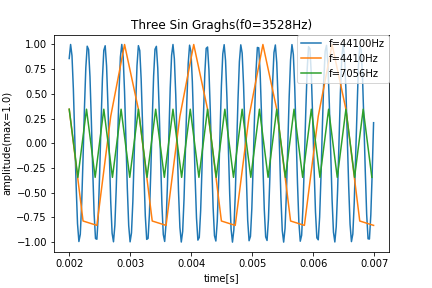
\includegraphics[height=70mm, width=150mm]{figures/two_sin_graghs.png}
 \caption{標本化周波数f0とf0/10の時の正弦波}
\end{figure}

この図からわかるように、標本化周波数が44100($>>3528\times 2$)Hzの時は正しく周波数3528Hzの正弦波を復元できており、また標本化周波数が7056Hzの時も先の例と比べるとズレが生じているが、周波数3528Hzの波を復元するという観点では依然として正しく復元できていると言える。しかし、標本化周波数4410($< 3528\times 2$)Hzの時は周波数$5\times 10^2$Hzの正弦波が復元されており、誤って復元されている。この時、周波数3528Hzの音とは異なる音が聞こえた。これは人が異なる周波数の音を別の音と捉えること(例えば音階)に起因する。ゆえに標本化定理で述べられるように、標本化するにはその波の周波数の2倍以上の標本化周波数が必要であることがわかる。また、標本化周波数が4410Hzの時に異なる波として復元され知覚される現象をエイリアシングと呼ぶ。さらに図1から標本化周波数7056Hzの時は振幅が小さくなっているが、確かに実験の際には7056Hzの時には44100Hzの時に比べて音が小さくなっていた。よって標本化周波数を定める際には標本化定理に留意しつつ、手に入れたい波形、調べたい性質に応じてより大きな標本化周波数で標本化する必要があると考えられる。

\section{参考文献}
[1] 電気情報工学科・電気電子工学科、「電気電子情報第一(前期)実験」、東京大学工学部(2019)

[2] 原島 博、「信号解析教科書 ー信号とシステムー」、コロナ社(2018)
\\
\end{document}
